%%%%%%%%%%%%%%%%%%%%%%%%%%%%%%%%% LAB-5 %%%%%%%%%%%%%%%%%%%%%%%%%%%%%%%%%%
%>>>>>>>>>>>>>>>>>>>>>>>>>> ПЕРЕМЕННЫЕ >>>>>>>>>>>>>>>>>>>>>>>>>>>>>>>>>>>
%>>>>> Информация о кафедре
%\newcommand{\year}{2021 г.}  % Год устанавливается автоматически
\newcommand{\city}{Санкт-Петербург}  %  Футер, нижний колонтитул на титульном листе
\newcommand{\university}{Национальный исследовательский университет ИТМО}  % первая строка
\newcommand{\department}{Факультет программной инженерии и компьютерной техники}  % Вторая строка
\newcommand{\major}{Направление системного и прикладного программного обеспечения}  % Треьтя строка
%<<<<< Информация о кафедре

%>>>>> Назание работы
\newcommand{\reporttype}{ОТЧЕТ ПО ЛАБОРАТОРНОЙ РАБОТЕ} % тип работы, (главный заголовок титульного листа)
\newcommand{\lab}{Лабораторная работа}          % вид работы
\newcommand{\labnumber}{№ 3}                    % порядковый номер работы
\newcommand{\subject}{Основы профессиональной деятельности}         % учебный предмет
\newcommand{\labtheme}{Исследование работы БЭВМ}            % Тема лабораторной работы
\newcommand{\variant}{№ 1024}                % номер варианта работы

\newcommand{\student}{Тюрин Иван Николаевич}    % определение ФИО студента
\newcommand{\studygroup}{P3110}                 % определение учебной группы 
\newcommand{\teacher}{Клименков С. В.,\\[1mm]     % ФИО лектора
                        Ларочкин Г. И.}          % ФИО практика
%<<<<<<<<<<<<<<<<<<<<<<<<<< ПЕРЕМЕННЫЕ <<<<<<<<<<<<<<<<<<<<<<<<<<<<<<<<<<<


%>>>>>>>>>>>>>>>>>>>>>> ПРЕАМБУЛА >>>>>>>>>>>>>>>>>>>>>>>>>

%>>>>>>>>>>>>>>>>>> ПРЕАМБУЛА >>>>>>>>>>>>>>>>>>>>
\documentclass[14pt,final,oneside]{extreport}% класс документа, характеристики
%>>>>> Разметка документа
\usepackage[a4paper, mag=1000, left=3cm, right=1.5cm, top=1cm, bottom=2cm, headsep=0.7cm, footskip=1cm]{geometry} % По ГОСТу: left>=3cm, right=1cm, top=2cm, bottom=2cm,
\linespread{1} % межстройчный интервал по ГОСТу := 1.5
%<<<<< Разметка документа

%>>>>> babel c языковым пакетом НЕ должны быть первым импортируемым пакетом
\usepackage[utf8]{inputenc}
\usepackage[T1,T2A]{fontenc}
\usepackage[russian]{babel}
%<<<<<

%\usepackage{cmap} %поиск в pdf

%>>>...>> прочие полезные пакеты
\usepackage{amsmath,amsthm,amssymb}
\usepackage{mathtext}
\usepackage{indentfirst}
\usepackage{graphicx}
\usepackage{float}
\graphicspath{{/home/ivan/itmo/informatics/latex}}
\DeclareGraphicsExtensions{.pdf,.png,.jpg}
%\usepackage{bookmark}

\usepackage[dvipsnames]{xcolor}
\usepackage{hyperref}  % Использование ссылок
\hypersetup{%  % Настройка разметки ссылок
    colorlinks=true,
    linkcolor=blue,
    filecolor=magenta,      
    urlcolor=magenta,
    %pdftitle={Overleaf Example},
    %pdfpagemode=FullScreen,
}
\usepackage{longtable}
\usepackage{diagbox}
\usepackage[letterspace=150]{microtype} % Спэйсинг (межбуквенный интервал для саголовка) \lsstyle

%>>> верстка в 2 колонки
\usepackage{multicol} % многоколоночная верстка
\setlength{\columnsep}{.15\textwidth} % определение ширины разделителя между колонками

%> кастомный разделитель колонок
\usepackage{tikz} % пакет для векторной графики, чтобы рисовать красивый разделитель колонок
\usetikzlibrary{arrows.meta,decorations.pathmorphing,backgrounds,positioning,fit,petri}
\usepackage{multicolrule} % Для кастомизации разделителя колонок
\SetMCRule{                     % кастомизация разделителя колонок multicolrule
    width=2pt,
    custom-line={               % Tikz код для кастомизации линии разделителя
        \draw [                 % Рисовать
            decorate,           % декорированную (требуются спец настройки пакетов tikz (см. импорт выше)
            decoration={        % вид декорирования
                snake, % Тип - змейка (волнистая)
                amplitude=.5mm, % ширина волн
                pre length=0mm, % участок прямой линии от начала
                %segment length=0mm, % учасок волнистой линии
                post length=0mm % участок прямой линии от конца
            },
            line width=1pt,
            step=10pt
        ] 
        (TOP) to (BOT); % сверху и до низа колонки
    }, 
    extend-top=-5pt, % Вылезти за верхнюю границу колонки 
    extend-bot=-7pt % Вылезти за нижнюю границу колонки  
}
%< кастомный разделитель колонок
%<<< верстка в 2 колонки

%>>>>> Использование листингов
\usepackage{listings} 
\usepackage{caption}
\DeclareCaptionFont{white}{\color{white}} 
\DeclareCaptionFormat{listing}{\colorbox{gray}{\parbox{\textwidth}{#1#2#3}}}

\captionsetup[lstlisting]{format=listing,labelfont=white,textfont=white} % Настройка вида описаний
\lstset{  % Настройки вида листинга
inputencoding=utf8, extendedchars=\true, keepspaces = true, % поддержка кириллицы и пробелов в комментариях
language={},            % выбор языка для подсветки (здесь это Pascal)
basicstyle=\small\sffamily, % размер и начертание шрифта для подсветки кода
numbers=left,               % где поставить нумерацию строк (слева\справа)
numberstyle=\tiny,          % размер шрифта для номеров строк
stepnumber=1,               % размер шага между двумя номерами строк
numbersep=5pt,              % как далеко отстоят номера строк от подсвечиваемого кода
backgroundcolor=\color{white}, % цвет фона подсветки - используем \usepackage{color}
showspaces=false,           % показывать или нет пробелы специальными отступами
showstringspaces=false,     % показывать илигнет пробелы в строках
showtabs=false,             % показывать или нет табуляцию в строках
frame=single,               % рисовать рамку вокруг кода
tabsize=2,                  % размер табуляции по умолчанию равен 2 пробелам
captionpos=t,               % позиция заголовка вверху [t] или внизу [b] 
breaklines=true,            % автоматически переносить строки (да\нет)
breakatwhitespace=false,    % переносить строки только если есть пробел
escapeinside={\%*}{*)}      % если нужно добавить комментарии в коде
}
%<<<<< Использование листингов
\usepackage{csvsimple} %импорт содержимого таблицы из csv


\sloppy % Решение проблем с переносами (с. 119 книга Львовского)
\emergencystretch=25pt


%>>>>>>>>>>>>>>>> ДОПОЛНИТЕЛЬНЫЕ КОМАНДЫ {Для соответствия ГОСТ} >>>>>>>>>>>>>>
%>>>>>> математические функции для удобства
\newcommand{\eps}{\varepsilon}
\newcommand{\limit}{\displaystyle\lim}
\newcommand{\oo}{\infty}
\newcommand{\Dx}{\Delta x}
\newcommand{\cd}{\cdot}
% \newcommand{\note}[2]{\overbrace{#1}^{#2}} % скобка сверху для комментария

%>>>>> Скобки
\newcommand{\lt}{\left}
\newcommand{\rt}{\right}
%<<<<< Скобки

%>>>>> Дроби
\newcommand{\cf}{\cfrac}
\newcommand{\fr}{\frac}
%<<<<< Дроби


%>>>>> Стрелки
\newcommand{\Rarr}{\Rightarrow}% ⇒ следствие
\newcommand{\LRarr}{\Leftrightarrow}% равносильно
\newcommand{\rarr}{\xrightarrow{}}% → стрелка вправо
\newcommand{\nwarr}{\nwarrow}% ↖ север-запад стрелка
\newcommand{\nearr}{\nearrow}% ↗ север-восток стрелка
\newcommand{\swarr}{\swarrow}% ↙ юг-запад стрелка
\newcommand{\searr}{\searrow}% ↘ юг-восток стрелка

\newcommand{\raises}{\nwarrow}% возрастает
\newcommand{\falls}{\swarrow}% убывает
\newcommand{\increases}{\nwarrow}% возрастает
\newcommand{\decreases}{\swarrow}% убывает

%{{{
\makeatletter
\newcommand{\xLeftrightarrow}[2][]{\ext@arrow 0359\Leftrightarrowfill@{#1}{#2}}% следствие с надписью
\makeatother
%}}}

%{{{
\makeatletter
\newcommand{\xRightarrow}[2][]{\ext@arrow 0359\Rightarrowfill@{#1}{#2}}% равносильность с надписью
\makeatother
%}}}
%<<<<< Стрелки
%>>>>> Стиль текста
\newcommand{\hex}[1]{\texttt{0{\footnotesize{x}}#1}}
\newcommand{\ttt}[1]{\texttt{#1}}
%<<<<< Стиль текста

%<<<<<< математические функции для удобства

\newcommand\Chapter[3]{%
    % Принимает 3 аргумента - название главы и дополнительный заголовок и ширина загловка (можно ничего)
    \refstepcounter{chapter}%
    \chapter*{%
        %\hfill % заполнение отступом пространства до заголовка
        \begin{minipage}{#3\textwidth} % Можно изменить ширину министраницы (заголовка)
            \flushleft % Выранивание заголовка по левому краю параграфа (заголовка)
            %\flushright % Выранивание заголовка по правому краю параграфа (заголовка)
            \begin{huge}%
                % Отключена нумерация глав в тексте:
                %:=% \textbf{\chaptername\ \arabic{chapter}\\}
                \textbf{#1}% Первый заголовок
            \end{huge}%
            \\% Перенос сторки
            \begin{Huge}
                #2% Второй заголовок
            \end{Huge}
        \end{minipage}
    }%
    % Отключена нумерация для chapter в toc (table of contents), т.е. Оглавлении (Содержании):
    %:=% \addcontentsline{toc}{chapter}{\arabic{chapter}. #1}
    % Представление главы в содержании:
    \addcontentsline{toc}{chapter}{#1. #2}%
}

\newcommand\Section[1]{
    % Принимает 1 аргумент - название секции
    \refstepcounter{section}
    \section*{%
        \raggedright
        % Отключена дополнительная нумерация chapter в section в тексте документа:
        %:=% \arabic{chapter}.\arabic{section}. #1}
        % Отключена любая нумарация section в тексте документа: (убрать \arabic{section}, оставить название секции)
        \arabic{section}. #1
    }
    
    % Отключена дополнительная нумерация chapter в section в toc (table of contents) Оглавлении (Содержании):
    %:=% \addcontentsline{toc}{section}{\arabic{chapter}.\arabic{section}. #1}
    \addcontentsline{toc}{section}{\arabic{section}. #1} 
}


\newcommand\Subsection[1]{
    % Принимает 1 аргумент - название подсекции
    \refstepcounter{subsection}
    \subsection*{%
        \raggedright%
        % Отключена дополнительная нумерация chapter в section в тексте документа (можно добавить отступ с помощью \hspace*{12pt}):
        %:=% \arabic{chapter}.\arabic{section}.\arabic{subsection}. #1}
        \arabic{section}. \arabic{subsection}. #1
    }
    % Отключена дополнительная нумерация chapter в section в Оглавлении (Содержании):
    %\addcontentsline{toc}{subsection}{\arabic{chapter}.\arabic{section}.\arabic{subsection}. #1}
    \addcontentsline{toc}{subsection}{\arabic{subsection}. #1}
}


\newcommand\Figure[4]{
    % Принимает 4 аргумента - название файла изображения, ее размер в тексте, описание, лэйбл (псевдоним в формате "fig:name") 
    %
    \refstepcounter{figure}
    \begin{figure}[H] %- \usepackage {float} %[h]
        \begin{center}
            \includegraphics[width=#2]{#1}
        \end{center}
        \caption{#3}
        \label{fig:#4}
    \end{figure}
}


\newcommand\Table[3]{
    % Принимает 3 аргумента --- лэйбл name(#1) (псевдоним в формате "tab:name"), ее описание(#2), содержание таблицы(#3) 
    %
    \refstepcounter{table}
    \renewcommand{\arraystretch}{1} % Установка высоты строки таблицы по умолчанию (=1), увеличенное на 0.2 пункта
    % \refstepcounter{table}% увеличение счетчика таблиц
    \begin{table}[htpb]% "right here"=H, "top", "new page", "bottom"
        \label{tab:#1}% лэйбл таблицы, для ссылок
        \resizebox{\columnwidth}{!}{% сжимает очень широкие таблицы, чтобы вместить на страницу
             #3% Содержание таблицы
        }
        % 
        \caption{#2}% Описание стандартными средствами для используемого окружения (table)
        % \captionof{table}{#2}% Описание стандартными средствами
        % \captionof*{figure}{\flushleft \textsc\textbf{Рис. 1.}}% Описание стандартными средствами, как рисунка
        %
        %%> кастомное описание
        % \begin{flushleft}% Кастомное описание
        %     % \textsf{%
        %         \textbf{%
        %             \\[2mm]
        %             #2% Описание к картинке
        %         }%
        %         % \\[8mm]% Отступ
        %     % }%
        % \end{flushleft}
        %%< кастомное описание
    \end{table}
    \renewcommand{\arraystretch}{1} % возврат установка высоты строки таблицы по умолчанию на 1
}


\newcommand\CustomFigure[4]{ % multicols не умеют в table и figure, поэтому приходится извращаться % вставка таблицы с меткой рисунка
    % Принимает 4 аргумента - название файла изображения, ее размер в тексте, описание, лэйбл (псевдоним в формате "fig:name") 
    %
    \refstepcounter{figure}
    \begin{figure}[ht]% "here", "top"
        \begin{center}
            \includegraphics[width=#2]{#1}
        \end{center}
        %
        %\caption{#3}
        \captionof{figure}{#3}% описание стандартными средствами
        % \begin{center}
        \begin{flushleft} % Кастомное описание
            \textbf{%
                #3% Текст описания
            }
        \end{flushleft}
        % \end{center}
        %
        \label{fig:#4}% Лэйбл, для ссылок
    \end{figure}
}


\newcommand\CustomTableFigure[3]{ % multicols не умеют в table и figure, поэтому приходится извращаться % вставка таблицы с меткой рисунка
    %
    % Принимает 3 аргумента --- лэйбл name(#1) (псевдоним в формате "tab:name"), ее описание(#2), содержание таблицы(#3) 
    %
    \begin{center}
        \refstepcounter{figure}
        \label{tab:#1}% лэйбл таблицы, для ссылок
        \resizebox{\columnwidth}{!}{% сжимает очень широкие таблицы, чтобы вместить на страницу
            #3% Содержание таблицы
        }
        % 
        \captionof{figure}{#2}% Описание стандартными средствами
        % \captionof*{figure}{\flushleft \textsc\textbf{Рис. 1.}}% Описание стандартными средствами
        %
        \begin{flushleft}% Кастомное описание
            % \textsf{%
                \textbf{%
                    \\[2mm]
                    #2% Описание к картинке
                }%
                % \\[8mm]% Отступ
            % }%
        \end{flushleft}
    \end{center}
}


\newcommand{\InkscapeFigure}[4]{% Вставки иллюстраций из Inkscape (pdf+latex)
    %
    % Принимает 4 параметра: #1 название файла, #2 описание, #3 лейбл #4 размер
    %
    % \begin{minipage}{#4}
        \begin{figure}[htbp]
            \centering
            \def\svgwidth{#4}
            \import{./figures/}{#1.pdf_tex}
            \caption{#2}
            \label{fig:#3}
        \end{figure}
    % \end{minipage}
}


\newcommand\Equation[3]{% Кастомное оформление выражений
    %
    % Принимает 3 аргумента --- лэйбл name (#1) (псевдоним в формате "tab:name"), его описание(#2), содержание выражения (#3) 
    %
    \textbf{#2}% описание
    \begin{equation}
        #3% содержимое выражений
        \label{eq:#1}% лэйбл
    \end{equation}
}

%<<<<<<<<<<<<<<<<<<<<<<<<<<<< ДОПОЛНИТЕЛЬНЫЕ КОМАНДЫ <<<<<<<<<<<<<<<<<<<<<<<<<<

%<<<<<<<<<<<<<<<<<<<<<< ПРЕАМБУЛА <<<<<<<<<<<<<<<<<<<<<<<<<



%%%%%%%%%%%%%%%%%%% СОДЕРЖИМОЕ ОТЧЕТА %%%%%%%%%%%%%%%%%%%%%
%>>>>>>>>>>>>>>> ''''''''''''''''''''''' >>>>>>>>>>>>>>>>>>
\begin{document}


%>>>>>>>>>>>>>>>> ОПРЕДЕЛЕНИЕ НАЗВАНИЙ >>>>>>>>>>>>>>>>>>>>
% Переоформление некоторых стандартных названий
%\renewcommand{\chaptername}{Лабораторная работа}
\renewcommand{\chaptername}{\lab\ \labnumber} % переименование глав
\def\contentsname{Содержание} % переименование оглавления
%<<<<<<<<<<<<<<<< ОПРЕДЕЛЕНИЕ НАЗВАНИЙ <<<<<<<<<<<<<<<<<<<<


%>>>>>>>>>>>>>>>>> ТИТУЛЬНАЯ СТРАНИЦА >>>>>>>>>>>>>>>>>>>>>
%>>>>>>>>>>>>>>>>>>> ТИТУЛЬНЫЙ ЛИСТ >>>>>>>>>>>>>>>>>>>>>>>
\begin{titlepage}

    % Название университета
    \begin{center}
    \textsc{%
        \university\\[5mm]
        \department\\[2mm]
        \major\\
    }

    \vfill
    \vfill
    % Название работы
    \textbf{\reporttype\ \labnumber\\[3mm]
    курса <<\subject>> \\[6mm]
    по теме: <<\labtheme>>\\[3mm]
    Вариант \variant\\[20mm]
    }
    \end{center}


\hfill
% Информация об авторе работы и проверяющем
\begin{minipage}{.5\textwidth}
    \begin{flushright}
        
            
        Выполнил студент:\\[2mm] 
        \student\\[2mm]
        группа: \studygroup\\[5mm]

        Преподаватель:\\[2mm] 
        \teacher

    \end{flushright}
\end{minipage}

\vfill

    % Нижний колонтитул первой страницы
    \begin{center}
        \city, \the\year\,г.
    \end{center}

\end{titlepage}
%<<<<<<<<<<<<<<<<<<< ТИТУЛЬНЫЙ ЛИСТ <<<<<<<<<<<<<<<<<<<<<<<


%<<<<<<<<<<<<<<<<< ТИТУЛЬНАЯ СТРАНИЦА <<<<<<<<<<<<<<<<<<<<<


%>>>>>>>>>>>>>>>>>>>>> СОДЕРЖАНИЕ >>>>>>>>>>>>>>>>>>>>>>>>>
% Содержание
\tableofcontents
%<<<<<<<<<<<<<<<<<<<<< СОДЕРЖАНИЕ <<<<<<<<<<<<<<<<<<<<<<<<<


%%%%%%%%%%%%%%%%%%%%%%% КОД РАБОТЫ %%%%%%%%%%%%%%%%%%%%%%%%
%>>>>>>>>>>>>>>>>>>>'''''''''''''''''>>>>>>>>>>>>>>>>>>>>>
\newpage
\Chapter{\lab\ \labnumber}{\labtheme}{}

\Section{Задание варианта \variant}
\begin{center}
, , ,
\end{center}
\noindent

\textit{По выданному преподавателем варианту восстановить текст заданного варианта программы, определить предназначение и составить описание программы, определить область представления и область допустимых значений исходных данных и результата, выполнить трассировку программы.}

\textit{Ход работы, содержание отчета и контрольные вопросы описаны в методических указаниях}

\begin{center}
    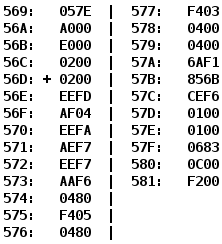
\includegraphics[width=0.3\paperwidth]{figures/task.png}
\end{center}
\begin{center}
    ' ' '
\end{center}

\newpage
\Section{Описание программы}

\Subsection{Назначение программы и реализуемые ею функция}

Описание программы представлено в таблице 1.1. %\ref{tab:program}.
В результате выполнения программы происходит подсчет элементов массива длины 4, которые не имеют остатка при делении на 4.
\Table{program}{Описание работы программы}{
    %\begin{longtable}{!t}
    \begin{tabular}{|l|l|l|l|}

\hline
\textbf{Адрес} & \textbf{\begin{tabular}[c]{@{}l@{}}Данные/\\ /Команда\end{tabular}} & \textbf{Мнемоника}                                                             & \textbf{Описание [, метка]}                                                                                                       \\ \hline
\hex{569}      & \hex{057e}                                                          & -                                                                              & Адрес начала массива \ttt{Y0}, \ttt{X1:}                                                                                          \\ \hline
\hex{56a}      & \hex{a000}                                                          & -                                                                              & \begin{tabular}[c]{@{}l@{}}Данные затираются значением \\ \ttt{X1=Y0}, по ним происходит \\ итерирование, \ttt{X2:}\end{tabular}  \\ \hline
\hex{56b}      & \hex{e000}                                                          & -                                                                              & \begin{tabular}[c]{@{}l@{}}Данные затираются значением \\ \hex{04}, количество элементов\\ массива, \ttt{X3:}\end{tabular}        \\ \hline
\hex{56c}      & \hex{0200}                                                          & -                                                                              & \begin{tabular}[c]{@{}l@{}}Данные обнуляются, счетчик\\ чисел кратных 4, \ttt{X4:}\end{tabular}                                   \\ \hline
\hex{56d}      & \hex{0200}                                                          & \ttt{cla}                                                                      & Очистка аккумулятора                                                                                                              \\ \hline
\hex{56e}      & \hex{eefd}                                                          & \ttt{st X4}                                                                    & Запись \ttt{AC} в \ttt{X4}                                                                                                        \\ \hline
\hex{56f}      & \hex{af04}                                                          & \ttt{ld \#\hex{04}}                                                            & Чтение в \ttt{AC} числа \hex{04}                                                                                                  \\ \hline
\hex{570}      & \hex{eefa}                                                          & \ttt{st X3}                                                                    & Запись \ttt{AC} в \ttt{X3}                                                                                                        \\ \hline
\hex{571}      & \hex{aef7}                                                          & \ttt{ld X1}                                                                    & Чтение в \ttt{AC} значения \ttt{X1}                                                                                               \\ \hline
\hex{572}      & \hex{eef7}                                                          & \ttt{st X2}                                                                    & Запись \ttt{AC} в \ttt{X2}                                                                                                        \\ \hline
\hex{573}      & \hex{aaf6}                                                          & \ttt{ld (X2)+}                                                                 & \begin{tabular}[c]{@{}l@{}}Автоинкрементное чтение в \\ \ttt{AC} из \ttt{X2}, и начало\\ цикла, \ttt{\_loop:}\end{tabular}         \\ \hline
\hex{574}      & \hex{0480}                                                          & \ttt{ror}                                                                      & \begin{tabular}[c]{@{}l@{}}Цикличиский сдвиг вправо, \\ \ttt{C} $=AC\ \mathrm{mod}\ 2$\end{tabular}                                 \\ \hline
\hex{575}      & \hex{f405}                                                          & \begin{tabular}[c]{@{}l@{}}\ttt{bhis \_endl}\\ (\ttt{blo \_endl})\end{tabular}  & \begin{tabular}[c]{@{}l@{}}Переход к концу цикла, если \\ \ttt{AC=Yi} не делится на 2\\ (\ttt{C=1})\end{tabular}                  \\ \hline
\hex{576}      & \hex{0480}                                                          & \ttt{ror}                                                                      & \begin{tabular}[c]{@{}l@{}}Цикличиский сдвиг вправо, \\ \ttt{C} $=AC\ \mathrm{mod}\ 2$\end{tabular}                                 \\ \hline
\hex{577}      & \hex{f403}                                                          & \begin{tabular}[c]{@{}l@{}}\ttt{bhis \_endl}\\ (\ttt{blo \_endl})\end{tabular} & \begin{tabular}[c]{@{}l@{}}Переход к концу цикла, если \\ \ttt{AC=Yi} не делится на 4 \\ (\ttt{C=1})\end{tabular}                 \\ \hline
\hex{578}      & \hex{0400}                                                          & \ttt{rol}                                                                      & Цикличиский сдвиг влево                                                                                                           \\ \hline
\hex{579}      & \hex{0400}                                                          & \ttt{rol}                                                                      & Цикличиский сдвиг влево                                                                                                           \\ \hline
\hex{57a}      & \hex{6af1}                                                          & \ttt{sub (X4)+}                                                                & \begin{tabular}[c]{@{}l@{}}Вычитание из \ttt{AC} значения \\ по адресу в \ttt{X4}, сдвиг указателя\\ \ttt{X4} вперед\end{tabular} \\ \hline
\hex{57b}      & \hex{856b}                                                          & \ttt{loop \$X3}                                                                & \begin{tabular}[c]{@{}l@{}}Уменьшение значения в \ttt{X3} до\\  нуля в цикле, конец цикла, \ttt{\_endl:}\end{tabular}             \\ \hline
\hex{57c}      & \hex{cef6}                                                          & \ttt{jump \_loop}                                                              & Переход к началу цикла \ttt{\_loop}                                                                                               \\ \hline
\hex{57d}      & \hex{0100}                                                          & \ttt{hlt}                                                                      & Останов                                                                                                                           \\ \hline
\hex{57e}      & \hex{0100}                                                          & -                                                                              & Первый элемент массива, \ttt{Y0:}                                                                                                 \\ \hline
\hex{57f}      & \hex{0683}                                                          & -                                                                              & Второй элемент массива                                                                                                            \\ \hline
\hex{580}      & \hex{0c00}                                                          & -                                                                              & Третий элемент массива                                                                                                            \\ \hline
\hex{581}      & \hex{f200}                                                          & -                                                                              & Четвертый элемент массива                                                                                                         \\ \hline
\end{tabular}

    %\end{longtable}
}
\Subsection{Область представления и допустимых значений}
Ограничения накладываются только на \ttt{X3}, количество элемнотов массива, так как их не может быть больше чем возможно разместить в памяти (\hex{800=2048}$-S$, где $S$ -- число команд в программе), и \ttt{X1}, так как он хранит адрес начала массива, значение которого не может превышать максимальный адрес \hex{7ff}.

Значения \ttt{X2} и \ttt{X4} не ограничены, потому что они затираются другими значениями в начале программы.

Значения элементов массива \ttt{Y} не ограничены, так как они используются только для определения делимости на 4, путем получения остатка по модулю 2 при цикличесом сдвиге вправо.

\Subsection{Трассировка программы}

Трассировка программы представлена в таблице 1.2.%\ref{tab:tracetable}.
\Table{tracetable}{Трассировка программы}{
    Адр & Знчн & IP  & CR   & AR  & DR   & SP  & BR   & AC   & NZVC & Адр & Знчн\\\hline
075 & 0200 & 075 & 0000 & 000 & 0000 & 000 & 0000 & 0000 & 0100 & &\\
075 & 0200 & 076 & 0200 & 075 & 0200 & 000 & 0075 & 0000 & 0100 & &\\
076 & EE19 & 077 & EE19 & 090 & 0000 & 000 & 0019 & 0000 & 0100 & 090 & 0000\\
077 & AE16 & 078 & AE16 & 08E & 00B8 & 000 & 0016 & 00B8 & 0000 & &\\
078 & 0700 & 079 & 0700 & 078 & 0700 & 000 & 0078 & 00B9 & 0000 & &\\
079 & 0C00 & 07A & 0C00 & 7FF & 00B9 & 7FF & 0079 & 00B9 & 0000 & 7FF & 00B9\\
07A & D694 & 694 & D694 & 7FE & 007B & 7FE & D694 & 00B9 & 0000 & 7FE & 007B\\
694 & AC01 & 695 & AC01 & 7FF & 00B9 & 7FE & 0001 & 00B9 & 0000 & &\\
695 & F204 & 696 & F204 & 695 & F204 & 7FE & 0695 & 00B9 & 0000 & &\\
696 & F003 & 697 & F003 & 696 & F003 & 7FE & 0696 & 00B9 & 0000 & &\\
697 & 7E09 & 698 & 7E09 & 6A1 & 00D0 & 7FE & 0009 & 00B9 & 1000 & &\\
698 & F005 & 699 & F005 & 698 & F005 & 7FE & 0698 & 00B9 & 1000 & &\\
699 & F804 & 69E & F804 & 699 & F804 & 7FE & 0004 & 00B9 & 1000 & &\\
69E & AE02 & 69F & AE02 & 6A1 & 00D0 & 7FE & 0002 & 00D0 & 0000 & &\\
69F & EC01 & 6A0 & EC01 & 7FF & 00D0 & 7FE & 0001 & 00D0 & 0000 & 7FF & 00D0\\
6A0 & 0A00 & 07B & 0A00 & 7FE & 007B & 7FF & 06A0 & 00D0 & 0000 & &\\
07B & 0800 & 07C & 0800 & 7FF & 00D0 & 000 & 007B & 00D0 & 0000 & &\\
07C & 4E13 & 07D & 4E13 & 090 & 0000 & 000 & 0013 & 00D0 & 0000 & &\\
07D & EE12 & 07E & EE12 & 090 & 00D0 & 000 & 0012 & 00D0 & 0000 & 090 & 00D0\\
07E & AE10 & 07F & AE10 & 08F & 00AA & 000 & 0010 & 00AA & 0000 & &\\
07F & 0C00 & 080 & 0C00 & 7FF & 00AA & 7FF & 007F & 00AA & 0000 & 7FF & 00AA\\
080 & D694 & 694 & D694 & 7FE & 0081 & 7FE & D694 & 00AA & 0000 & 7FE & 0081\\
694 & AC01 & 695 & AC01 & 7FF & 00AA & 7FE & 0001 & 00AA & 0000 & &\\
695 & F204 & 696 & F204 & 695 & F204 & 7FE & 0695 & 00AA & 0000 & &\\
696 & F003 & 697 & F003 & 696 & F003 & 7FE & 0696 & 00AA & 0000 & &\\
697 & 7E09 & 698 & 7E09 & 6A1 & 00D0 & 7FE & 0009 & 00AA & 1000 & &\\
698 & F005 & 699 & F005 & 698 & F005 & 7FE & 0698 & 00AA & 1000 & &\\
699 & F804 & 69E & F804 & 699 & F804 & 7FE & 0004 & 00AA & 1000 & &\\
69E & AE02 & 69F & AE02 & 6A1 & 00D0 & 7FE & 0002 & 00D0 & 0000 & &\\
69F & EC01 & 6A0 & EC01 & 7FF & 00D0 & 7FE & 0001 & 00D0 & 0000 & 7FF & 00D0\\
6A0 & 0A00 & 081 & 0A00 & 7FE & 0081 & 7FF & 06A0 & 00D0 & 0000 & &\\
081 & 0800 & 082 & 0800 & 7FF & 00D0 & 000 & 0081 & 00D0 & 0000 & &\\
082 & 0700 & 083 & 0700 & 082 & 0700 & 000 & 0082 & 00D1 & 0000 & &\\
083 & 4E0C & 084 & 4E0C & 090 & 00D0 & 000 & 000C & 01A1 & 0000 & &\\
084 & EE0B & 085 & EE0B & 090 & 01A1 & 000 & 000B & 01A1 & 0000 & 090 & 01A1\\
085 & AE07 & 086 & AE07 & 08D & FFFF & 000 & 0007 & FFFF & 1000 & &\\
086 & 0C00 & 087 & 0C00 & 7FF & FFFF & 7FF & 0086 & FFFF & 1000 & 7FF & FFFF\\
087 & D694 & 694 & D694 & 7FE & 0088 & 7FE & D694 & FFFF & 1000 & 7FE & 0088\\
694 & AC01 & 695 & AC01 & 7FF & FFFF & 7FE & 0001 & FFFF & 1000 & &\\
695 & F204 & 69A & F204 & 695 & F204 & 7FE & 0004 & FFFF & 1000 & &\\
69A & 4C01 & 69B & 4C01 & 7FF & FFFF & 7FE & 0001 & FFFE & 1001 & &\\
69B & 4C01 & 69C & 4C01 & 7FF & FFFF & 7FE & 0001 & FFFD & 1001 & &\\
69C & 4E05 & 69D & 4E05 & 6A2 & 00B7 & 7FE & 0005 & 00B4 & 0001 & &\\
69D & CE01 & 69F & CE01 & 69D & 069F & 7FE & 0001 & 00B4 & 0001 & &\\
69F & EC01 & 6A0 & EC01 & 7FF & 00B4 & 7FE & 0001 & 00B4 & 0001 & 7FF & 00B4\\
6A0 & 0A00 & 088 & 0A00 & 7FE & 0088 & 7FF & 06A0 & 00B4 & 0001 & &\\
088 & 0800 & 089 & 0800 & 7FF & 00B4 & 000 & 0088 & 00B4 & 0001 & &\\
089 & 0740 & 08A & 0740 & 089 & 0740 & 000 & 0089 & 00B3 & 0001 & &\\
08A & 4E05 & 08B & 4E05 & 090 & 01A1 & 000 & 0005 & 0254 & 0000 & &\\
08B & EE04 & 08C & EE04 & 090 & 0254 & 000 & 0004 & 0254 & 0000 & 090 & 0254\\
08C & 0100 & 08D & 0100 & 08C & 0100 & 000 & 008C & 0254 & 0000 & &\\

}
\Section{Сокращенная программа}
Была составлена укороченная программа на языке ассемблера, дающая точно такой же результат, что и данная в варианте. Она представлена в листинге \ref{lst:improved}.

\refstepcounter{lstlisting}
\begin{figure}[H] %- \usepackage {float} %[h]
    \begin{center}
        \lstinputlisting[]{script-meaning.asm}
    \end{center}
    \captionof{lstlisting}{Код сокращенной программы}
    \label{lst:improved}
\end{figure}

\Section{Вывод}
\textbf{Вывод:} научился читать коды БЭВМ, сдерживать ярость, читать презентации и мысли лектора. Научился писать программы с ветвлениями на ассемблере БЭВМ.
% Вывод...
\newpage
%<<<<<<<<<<<<<<<<<<<<<< КОД РАБОТЫ <<<<<<<<<<<<<<<<<<<<<<<<


%>>>>>>>>>>>>>>>> СПИСОК ЛИТЕРАТУРЫ >>>>>>>>>>>>>>>>>>>>>>>
%
\bibliographystyle{plain}

\begin{thebibliography}{3}
    \addcontentsline{toc}{chapter}{Список лиетратуры}

    \bibitem{gutgut:1}
    Код Хэмминга. Пример работы алгоритма. URL: \url{https://habr.com/ru/post/140611/};

    \bibitem{gutgut:2}
    Избыточное кодирование, код Хэмминга. URL: \url{https://neerc.ifmo.ru/wiki/index.php?title=%D0%98%D0%B7%D0%B1%D1%8B%D1%82%D0%BE%D1%87%D0%BD%D0%BE%D0%B5_%D0%BA%D0%BE%D0%B4%D0%B8%D1%80%D0%BE%D0%B2%D0%B0%D0%BD%D0%B8%D0%B5,_%D0%BA%D0%BE%D0%B4_%D0%A5%D1%8D%D0%BC%D0%BC%D0%B8%D0%BD%D0%B3%D0%B0}.

\end{thebibliography}  % Для соответсвия гост, придется доработать. Нужен файл .bib
%<<<<<<<<<<<<<<<<<<<< СПИСОК ЛИТЕРАТУРЫ <<<<<<<<<<<<<<<<<<<


\end{document}
%<<<<<<<<<<<<<<<< ,,,,,,,,,,,,,,,,,,,,,,, <<<<<<<<<<<<<<<<<
%<<<<<<<<<<<<<<<<<<< СОДЕРЖИМОЕ ОТЧЕТА <<<<<<<<<<<<<<<<<<<<
